%************************************************
\chapter{Un modèle morphologique de scènes sonores environnementales}\label{ch:psycho_model} % $\mathbb{ZNR}$
%************************************************

\section{Motivations}

étude de la contribution des sources sonores \\

G1: \citep{bruce2009development,bruce2014effects}; \\
G2: \citep{davies2014soundscape} montre que quand on demande à des participants de simuler un paysage sonore, les simulations font références à ce que les participants s'imaginent être un environnement typique, sans tenir compte de leur propre préférence pour des sons particuliers.

\section{Un modèle morphologique}

\subsection{Inspiration perceptive}

\subsection{Formalisation du modèle}

\section{Du modèle à la simulation dans le cadre de l'analyse sensorielle: l'outil \emph{Simscene}}

\subsection{Proposition d'un protocole expérimental basé sur la simulation}

\subsubsection{Paradigme}

\subsubsection{Contraintes}

\subsection{Organisation des sons isolées}
\label{db_ui}

Pour les événements, les regroupements se font en grande majorité par rapport à la source et sont d’ordre sémantique. Pour les textures nous considérons également la morphologie des lieux hébergeant ces dernières.

\begin{figure}[bth]
        \myfloatalign
        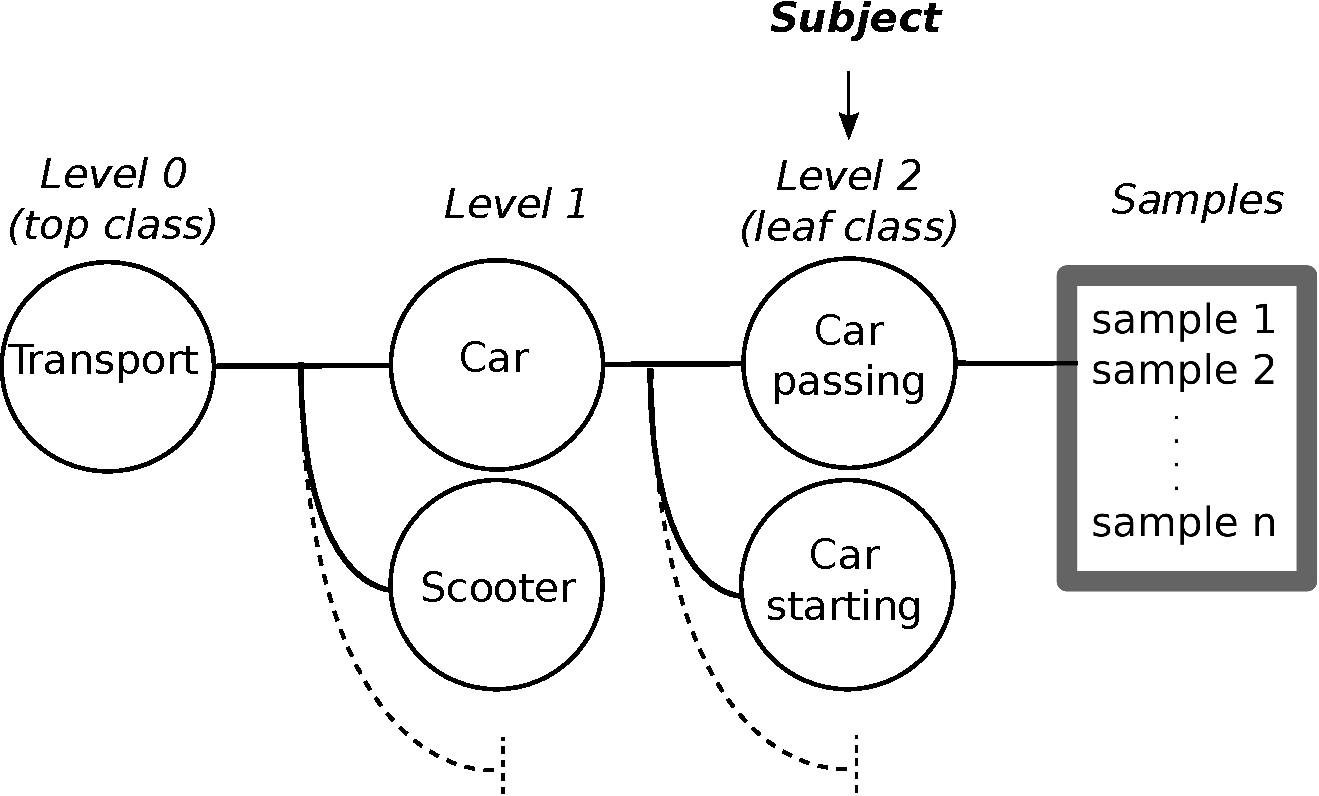
\includegraphics[width=.8\linewidth]{gfx/3-eps-converted-to}
       \caption{Organisation hiérarchique de la banque de sons isolés utilisée pour la simulation}\label{fig:orgDb}
\end{figure}

\subsection{Sélection des sons isolés}

\subsection{Processus de simulation et paramètres de contrôle}

%*****************************************
%*****************************************
%*****************************************
%*****************************************
%*****************************************
